\documentclass[a4paper,11pt]{article}
\usepackage{amssymb}
\usepackage[polish]{babel}
\usepackage[utf8]{inputenc}
\usepackage[T1]{fontenc}
\usepackage{graphicx}
\usepackage{anysize}
\usepackage{enumerate}
\usepackage{times}
\usepackage{geometry}
\usepackage{amsthm}
\usepackage{pgfplots}

\usepackage[intlimits]{amsmath}
\marginsize{3cm}{3cm}{1.5cm}{1.5cm}
\sloppy

\begin{document}
\begin{table}[ht]
\centering
\hspace*{-1cm}
\begin{tabular}{lllllll}
\cline{1-6}
\multicolumn{1}{|c|}{\begin{tabular}[c]{@{}c@{}}EAIiIB\\ Informatyka\end{tabular}}              & \multicolumn{2}{l|}{\begin{tabular}[c]{@{}l@{}}Aleksander Lisiecki\\ Natalia Materek\end{tabular}}                                                                                                & \multicolumn{1}{c|}{\begin{tabular}[c]{@{}c@{}}Rok\\ II\end{tabular}}          & \multicolumn{1}{c|}{\begin{tabular}[c]{@{}c@{}}Grupa\\ 2\end{tabular}}            & \multicolumn{1}{c|}{\begin{tabular}[c]{@{}c@{}}Zespół\\ 6\end{tabular}}      &  \\ \cline{1-6}
\multicolumn{1}{|c|}{\begin{tabular}[c]{@{}c@{}}Pracownia\\ FIZYCZNA\\ WFiIS AGH\end{tabular}} & \multicolumn{4}{l|}{\begin{tabular}[c]{@{}l@{}}Temat:\\ \textbf{\textit{Elektroliza}} \end{tabular}}                                                                                                                                                                                                                                            & \multicolumn{1}{c|}{\begin{tabular}[c]{@{}c@{}}Nr ćwiczenia:\\ 35\end{tabular}} &  \\ \cline{1-6}
\multicolumn{1}{|l|}{\begin{tabular}[c]{@{}c@{}}Data wykonania:\\ 20.12.2016\end{tabular}}      & \multicolumn{1}{c|}{\begin{tabular}[c]{@{}c@{}}Data oddania:\\ 04.01.2017\end{tabular}} & \multicolumn{1}{l|}{\begin{tabular}[c]{@{}l@{}}Zwrot do poprawki:\\ \phantom{data poprawki}\end{tabular}} & \multicolumn{1}{l|}{\begin{tabular}[c]{@{}l@{}}Data oddania:\\  \phantom{data oddania}\end{tabular}} & \multicolumn{1}{l|}{\begin{tabular}[c]{@{}l@{}}Data zaliczenia:\\  \phantom{data zaliczenia}\end{tabular}} & \multicolumn{1}{l|}{\begin{tabular}[c]{@{}l@{}}OCENA:\\ \phantom{ocena}\end{tabular}}       &  \\ \cline{1-6}
                                                                                                
\end{tabular}
\end{table}

\begin{center}
\begin{LARGE}
\textbf{Ćwiczenie nr 35: Elektroliza}
\end{LARGE}
\end{center}

\section{Cel ćwiczenia}

\indent Wyznaczanie równoważnika  elektrochemicznego    miedzi    oraz    stałej    Faradaya w doświadczeniu z~elektrolizą wodnego roztworu $\text{CuSO}_4$

\section{Wstęp teoretyczny}
\indent Elektroliza zachodzi w układach, w których występują substancje zdolne do jonizacji, czyli rozpadu na jony. Samo zjawisko jonizacji może być wywołane zarówno przyłożonym napięciem elektrycznym, jak i zjawiskami nie generowanymi bezpośrednio przez prąd – dysocjacją elektrolityczną, autodysocjacją, wysoką temperaturą czy działaniem silnego promieniowania.

\indent By zobojętnić jon na elektrodzie, musi przepłynąć ładunek równy $w \cdot e$, gdzie $e$ - ładunek elementarny elektronu [$C$], a $w$ - wartościowość jonu.
Liczbę atomów które wydzieliły się na elektrodzie możemy wyznaczyć jako stosunek całkowitego ładunku ($I\cdot t$) do ładunku pojedynczego jonu ($w \cdot e$)
\begin{equation}
N=\frac{It}{we}
\end{equation}
gdzie
\begin{description}
\item [$I$] natężenie płynącego prądu [$A$]
\item [$t$] czas przepływu prądu [$s$]
\item [$w$] wartościowość jonu [bezwymiarowa]
\item [$e$] ładunek elementarny elektronu [$C$]
\end{description}

\indent Aby obliczyć masę osadzonych atomów, mnożymy ich ilość przez masę jednego atomu. Masę pojedynczego atomu można wyznaczyć jako stosunek masy molowej do
liczby Avogadra, stąd
\begin{equation}
\label{eq:masa}
m=N\frac{\mu}{N_A}=\frac{\mu}{weN_A}It
\end{equation}
gdzie
\begin{description}
\item [$\mu$] masa molowa jednego atomu substancji [$g$]
\item [$N_{A}$] liczba Avogadra [$mol$]
\item [$N$] liczba atomów
\end{description}

\indent Zauważamy, że masa wydzielonej substancji jest proporcjonalna do natężenia prądu $I$, czasu przepływu prądu $t$ oraz współczynnika oznaczanego $k$ i zwanego elektrochemicznym równoważnikiem substancji.
\begin{equation}
\label{eq:k}
k=\frac{\mu}{weN_A}
\end{equation}
gdzie 
\begin{description}
\item [$k$] elektrochemiczny równoważnik substancji [$\frac{kg}{C}$]
\end{description}

\indent Iloczyn $eN_A$ wyraża ładunek potrzebny do wydzielenie jednego gramorównoważnika chemicznego substancji. Oznacza się go zwykle jako $F$ i nazywa stałą Faradaya.
Ze wzoru (\ref{eq:k}) wynika jego zależność od $k$:
\begin{equation}
\label{eq:F}
F=\frac{\mu}{wk}
\end{equation}
gdzie 
\begin{description}
\item [$F$] to stała Faradaya [$\frac{C}{mol}$]
\end{description}

\indent Nie należy mylić elektrolizy z procesami zachodzącymi w ogniwie galwanicznym. W elektrolizie energia elektryczna zamieniana jest na chemiczną, a w ogniwie galwanicznym kierunek przemian energetycznych jest przeciwny, tzn. energia chemiczna w procesie reakcji redoks zamieniana jest na energię elektryczną, co objawia się generowaniem prądu w obwodzie łączącym elektrody ogniwa. Ze względu na odwrotny przebieg procesu w ogniwach galwanicznych katoda jest naładowana dodatnio, a anoda ujemnie, jednak procesy chemiczne zachodzące na obu ogniwach mają podobny charakter.

\section{Układ pomiarowy}
\begin{figure}[h!]
\label{rys:1}
\centering
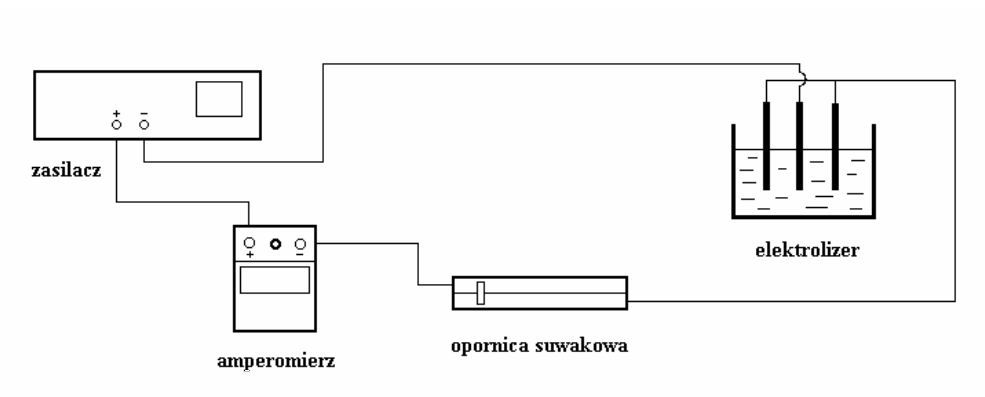
\includegraphics[width=0.7\linewidth]{./uklad}
\caption{Schemat obwodu elektrycznego}
\label{fig:uklad}
\end{figure}

\subsubsection*{Przyrządy}
Układ pomiarowy został przedstawiony na rysunku 1.
\begin{itemize}
\item Naczynie do elektrolizy siarczanu miedzi $\text{CuSO}_4$ z miedzianymi elektrodami w kształcie
równoległych płyt, oddalonych od siebie o kilka centymetrów
\item Zasilacz napięcia stałego
\item Amperomierz
\item Opornica suwakowa
\item Waga elektroniczna
\end{itemize}


\section{Wyniki pomiarów}
\begin{center}
\begin{tabular}{lrlll}
czas elektrolizy               & $t$ & = & 35 & min  \\ 
natężenie prądu               &  $I$ & = & 0,515 & A \\ 
masa katody przed elektrolizą &  $m_1$ & = & 72,817 & g \\ 
masa katody po elektrolizie  &   $m_2$ & = & 73,185 & g\\ 
masa wydzielonej miedzi       &  $m = m_2 - m_1$& = & 0,368 & g \\ 
masa anod przed elektrolizą   &   ${M_1}_{A}$ & = &225,321 & g\\ 
  &   ${M_1}_{B}$ & = &122,350 & g\\ 
masa anod po elektrolizie     &   ${M_2}_{A}$ & = &224,984 & g\\
  &   ${M_2}_{B}$ & = &122,213 & g\\  
zmiana masy anod               &  $M = M_2 - M_1$& = & 0,337 & g \\  
\end{tabular} 
\end{center}

\subsection*{Dane określające niepewność przyrządów:}
\begin{center}
\begin{tabular}{lrlll}
Klasa amperomierza              & &  & 0,5 &   \\ 
Używany zakres amperomierza               &   & 0 & 0,75 & A \\ 
Niepewność graniczna wagi (znamionowa)&  $\Delta m$ & = & 0,001 & g \\ 
Niepewność pomiaru masy &   $u(m)$& = & 0,00058 & g\\  
\end{tabular} 
\end{center}

\section{Opracowanie wyników}
Aby obliczyć współczynnik elektrochemiczny $k$ korzystamy ze wzoru:
\begin{equation}
k = \frac{m}{It}
\end{equation}
$$
k = \frac{m}{I t} = \frac{0,368}{0,515 \cdot 35 \cdot 60} \frac{g}{A \cdot s}  = 0,3403 \cdot 10^{-3} \frac{g}{A \cdot s} 
$$
Korzystając z otrzymanej wartości współczynnika  $k$ i  wzoru obliczamy doświadczalną wartość stałej Faradaya ze wzoru {\ref{eq:F}}:
$$
F = \frac{\mu}{w k} = \frac{63,58 }{2 \cdot 0,3403 \cdot 10^{-3}} \frac{C}{mol} = 93418~\frac{C}{mol}, 
$$
gdzie 
\begin{description}
\item [$\mu$] to masa molowa miedzi równa $63,58 ~\dfrac{g}{mol}$
\item [$w$] to wartościowość miedzi równa 2.
\end{description}

Korzystając z otrzymanej wartości stałej Faradaya  $F$, obliczamy doświadczalną wartość ładunku elementarnego ze wzoru:
\begin{equation}
e = \frac{F}{N_A}
\end{equation}

$$
e = \frac{F}{N_A} = \frac{93418}{6,0222 \cdot 10^{23}}~C = 1,551 \cdot 10^{-19}~C,  
$$
gdzie $N_A$ to liczba Avogadra, która jest wielkością stałą informującą o liczbie cząsteczek lub atomów zawartych w jednym molu substancji. 

\section{Obliczanie niepewności pomiarowej}
\indent Za niepewność pomiaru czasu przyjęto $u(t)=3s$, ze względu na opóźnioną reakcję przy włączaniu stopera. 

\indent Mimo, iż niepewność graniczna pomiaru wagi wynosiła 0,001g przyjęto ją jako:
$$
u(m) = 0,005 g
$$
Biorąc pod uwagę nieuniknione błędy w trakcie wykonania doświadczenia tj. niedokładnego wysuszenia elektrod, niedokładne przepłukanie elektrod lub zanieczyszczenia samego elektrolitu.

\indent Aby policzyć niepewność wartości ładunku elektrycznego, który przepłynął przez elektrolit musimy znać niepewność pomiaru natężenia:
\begin{equation}
u(I) = \frac{\text{klasa amperomierza} \cdot \text{zakres}}{100}
\end{equation}
gdzie 
\begin{description}
\item [$u(I)$] niepewność wartości natężenia prądu [$A$]
\end{description}
Podstawiając do wzoru otrzymujemy:
$$
u(I) = \frac{0,5 \cdot 0,75}{100} = 0,0038
$$

Niepewność pomiaru ładunku elektrycznego:
\begin{equation}
\label{wzor:ue}
u(e) = t \cdot u(I)
\end{equation}
gdzie 
\begin{description}
\item [$u(e)$] niepewność pomiaru ładunku elektrycznego [$C$]
\end{description}

A zatem korzystając ze wzoru {\ref{wzor:ue}} niepewność wartości ładunku elektrycznego wynosi:
$$
u(e) = 2100 \cdot 0,0028 = 5,88 ~C
$$

\subsubsection*{Niepewność względna i bezwzględna  równoważnika elektrochemicznego}  

$$
\frac{u(k)}{k} = \sqrt{\left[\frac{u(m)}{m} \right]^2 + \left[\frac{u(I)}{I} \right]^2 } = \sqrt{\left[\frac{ 0,005}{0,368} \right]^2 + \left[\frac{0,0038}{0,515} \right]^2 } \approx 0,015
$$

gdzie
\begin{description}
\item [$u(k)$] niepewność bezwzględna równoważnika elektrochemicznego $\left[\frac{kg}{C}\right]$
\item [$k$] równoważnik elektrochemiczny substancji $\left [\frac{kg}{C}\right] $
\item [$u(m)$] niepewność pomiaru masy $[kg]$
\item [$m$] masa wydzielonej podczas elektrolizy miedzi $[kg]$
\item [$u(I)$] niepewność natężenia prądu płynącego podczas elektrolizy $[A]$
\item [$I$] natężenie prądu podczas elektrolizy $[A]$
\end{description}
$$
u(k) = \frac{u(k)}{k} \cdot k =  0,015 \cdot 0,3403 \cdot 10^{-3} \approx 0,0051 \cdot 10^{-3} ~ \frac{g}{A \cdot s}
$$

\subsubsection*{Niepewność względna i bezwzględna  stałej Faradaya oraz ładunku elementarnego}

$$
\frac{u(F)}{F} = \sqrt{\left[\frac{u(\mu)}{\mu} \right]^2 + \left[\frac{u(k)}{k} \right]^2 } = \sqrt{\left[\frac{u(k)}{k} \right]^2 } = \frac{u(k)}{k}  =   \frac{u(e)}{e}
$$
gdzie
\begin{description}
\item [$U(F)$] niepewność bezwzględna stałej Faradaya $\left[\frac{C}{mol} \right]$
\item [$F$] stała Faradaya $\left[\frac{C}{mol} \right]$
\item [$u(\mu)$] niepewność masy molowej miedzi $\left[\frac{g}{mol}\right]$
\item [$\mu$] masa molowa miedzi $\left[\frac{g}{mol}\right]$
\item [$u(e)$] niepewność wyznaczonego ładunku elementarnego [$C$]
\item [$e$] wartość wyznaczonego ładunku elementarnego [$C$]
\end{description}
$$
u(F) = F \frac{u(k)}{k}  =  94318  \cdot  0,015 = 1401,27  ~ \frac{C}{mol} 
$$

$$
u(e) = e \frac{u(k)}{k}  =  1,551 \cdot 10^{-19}  \cdot   0,015  = 0,023 \cdot 10^{-19} ~C 
$$

\section{Podsumowanie wyników}

\begin{tabular}{|l|p{2cm}|p{2,2cm}| p{2cm}| p{2cm} | p{2,2cm}|}
\hline  & wartość tablicowa  & wartość wyznaczona & różnica & niepewność  & niepewność względna [\%]  \\ 
\hline $k \left[  \frac{mg}{A \cdot s}\right]$ & 0,329  & 0,3403  & 0,013 & 0,0051 & 1,5  \\ 
\hline $F \left[  \frac{C}{mol}\right]$ & 96500 & 93418  & 3082  & 1401,27  & 1,5  \\ 
\hline $e [10^{-19} C]$ & 1,602   & 1,551    & 0,051 & 0,023   & 1,5  \\ 
\hline 
\end{tabular} 

\section{Wnioski}
\begin{itemize}

\item Masa anod uległa zmniejszeniu, a masa katody zwiększeniu. 
\item Wyznaczone wielkości stałej Faradaya, równoważnika elektrochemicznego miedzi oraz ładunku elementarnego nie mieszczą się w granicach błędu. Wyjaśnia to zapewne możliwość powstanie sporego błędu przypadkowego, jak np. niedokładne wysuszenie płytek, niedokładne ich opłukanie lub zanieczyszczenie elektrolitu. 
\item Elektrolity mogą być dobrymi przewodnikami. 
 
\end{itemize}

\end{document}